%# -*- coding:utf-8 -*-
\subsection[心脏分割]{基于测地学活动轮廓的心脏近似区域的分割}

\begin{frame}
\begin{itemize}
  \item \textbf{心脏区域前面观}:
\end{itemize}
\begin{figure}[t]
\centering
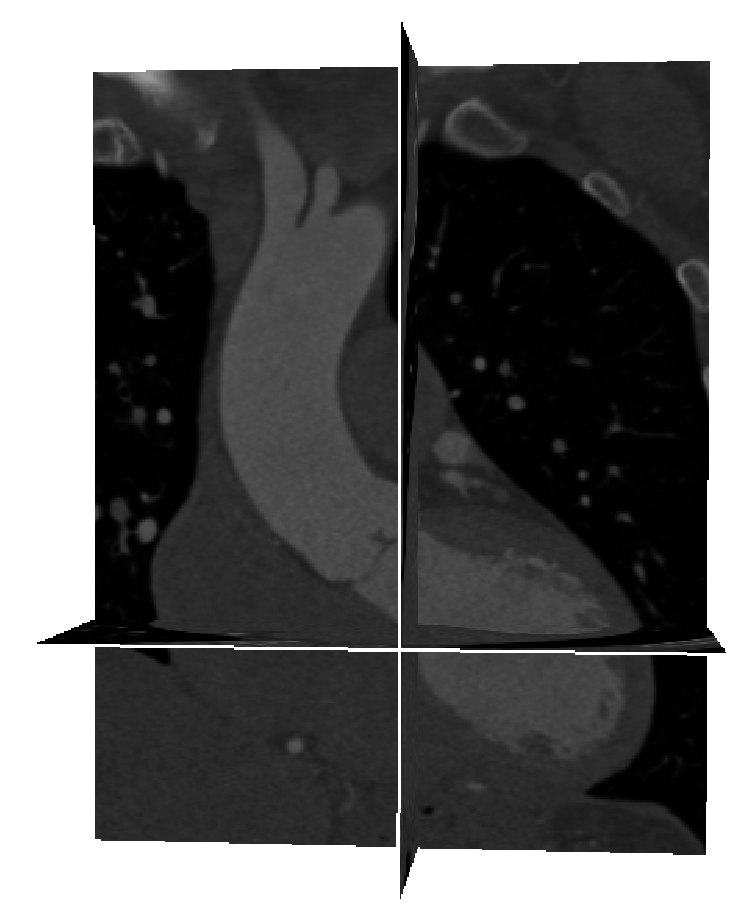
\includegraphics[height=1.5in]{../../Figures/gac/heart/original.eps}
\end{figure}
\end{frame}

\begin{frame}
\begin{itemize}
  \item \textbf{心脏区域分割流程}:
\end{itemize}
\begin{figure}[t]
\centering
%# -*- coding:utf-8 -*-
\begin{tikzpicture}[scale=.3]

\draw [black,thick,rounded corners] (-3,0) rectangle (3,2);            % binary threshold
\draw [black,thick,rounded corners] (-3,3) rectangle (3,5);  % GAC

\draw [black,thick,rounded corners] (-8,7) rectangle (-2,9); % fast marching
\draw [black,thick,rounded corners] (-8,13) rectangle (-2,15); % thresholding
\draw [black,thin,dashed] (-8.5,6.5) rectangle (-1.5,15.5);
\node [above right] at (-8.5,15.5) {\tiny \fs \bf 初始水平集};

\draw [black,thick,rounded corners] (2,7) rectangle (8,9);   % sigmoid
\draw [black,thick,rounded corners] (2,10) rectangle (8,12); % gradient
\draw [black,thick,rounded corners] (2,13) rectangle (8,15); % curvature anisotropic diffusion
\draw [black,thin,dashed] (1.5,6.5) rectangle (8.5,15.5);
\node [above right] at (5,15.5) {\tiny \fs \bf 特征图像};

\draw [black,thick,rounded corners] (-3,17) rectangle (3,19); % raw input

\node [above right] at (-2.1,0.25) {\tiny \fs \bf 二值阈值滤波};
\node [above right] at (-2.1,3.25) {\tiny \fs \bf 测地活动轮廓};

\node [above right] at (-6.75,7.25) {\tiny \fs \bf 快速行进};
\node [above right] at (-6.75,13.25) {\tiny \fs \bf 阈值滤波};

\node [above right] at (2.3,7.25) {\tiny \fs \bf 亮度的非线性映射};
\node [above right] at (3,10.25) {\tiny \fs \bf 梯度幅值计算};
\node [above right] at (2.3,13.25) {\tiny \fs \bf 曲率各向异性扩散};

\node [above right] at (-1.9,17.25) {\tiny \fs \bf 原始体数据};

\draw [<-,thick] (0,2) -- (0,3);

\draw [<-,thick] (0,5) -- (0,6);
\draw [thick] (-5,6) -- (5,6);
\draw [thick] (-5,6) -- (-5,7);
\draw [thick] (5,6) -- (5,7);

\draw [<-,thick] (-5,9) -- (-5,13);
\draw [<-,thick] (5,9) -- (5,10);

\draw [<-,thick] (5,9) -- (5,10);
\draw [<-,thick] (5,12) -- (5,13);

\draw [<-,thick] (-5,15) -- (-5,16);
\draw [<-,thick] (5,15) -- (5,16);
\draw [thick] (-5,16) -- (5,16);
\draw [thick] (0,16) -- (0,17);

\end{tikzpicture} 
% 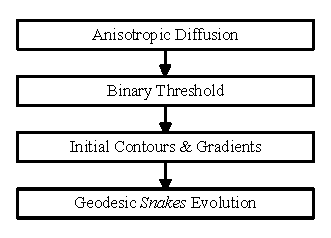
\includegraphics[height=2.0in]{figures/heart/DataFlow.eps}
% \caption[心脏区域分割流程]{心脏区域分割流程。}
% \label{fig:heart_data_flow}
\end{figure}
\end{frame}

\begin{frame}
\begin{itemize}
  \item \textbf{二值阈值后心脏区域前面观}:
  \begin{itemize}
    \item $\text{TH}_{\text{lower}} = 0$,$\text{TH}_{\text{upper}} = 200$
    \item 注意其中的心包,以及大部分血管等都已被除去
  \end{itemize}
\end{itemize}
\begin{figure}[t]
\centering
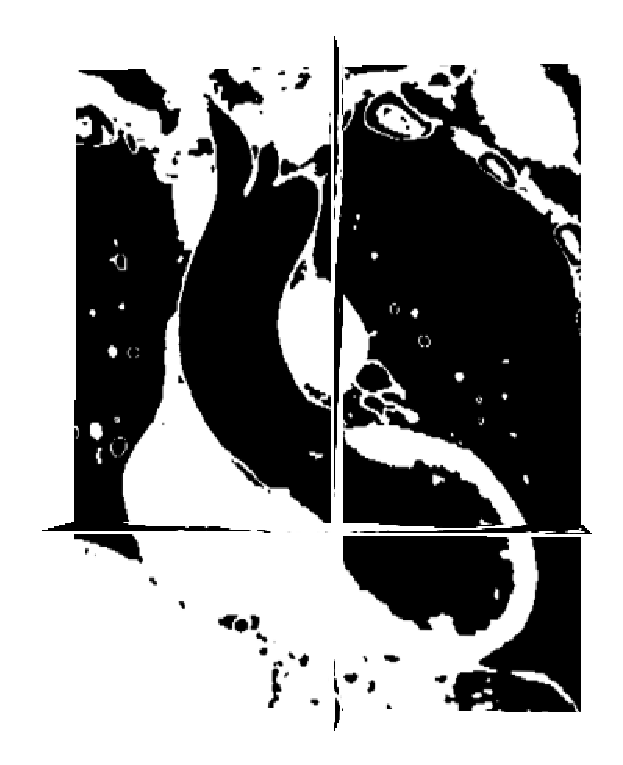
\includegraphics[height=1.5in]{../../Figures/gac/heart/binary_threshold.eps}
% \caption[二值阈值后心脏区域前面观]{二值阈值后心脏区域前面观($\text{TH}_{\text{lower}} = 0$,$\text{TH}_{\text{upper}} = 200$)。注意其中的心包,以及大部分血管等都已被除去。}%
% \label{fig:heart_binary_threshold_experiments}
\end{figure}
\end{frame}

\begin{frame}
\begin{itemize}
  \item \textbf{心脏表面模型前面观}:
  % \begin{itemize}
    % \item $\text{TH}_{\text{lower}} = 0$,$\text{TH}_{\text{upper}} = 200$
    % \item 注意其中的心包,以及大部分血管等都已被除去
  % \end{itemize}
\end{itemize}
\begin{figure}[t]
\centering
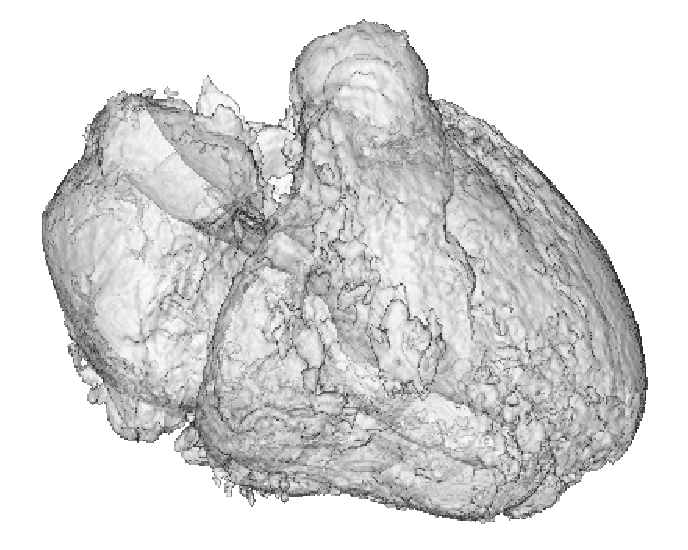
\includegraphics[height=1.5in]{../../Figures/gac/heart/heart.eps}
% \caption[二值阈值后心脏区域前面观]{二值阈值后心脏区域前面观($\text{TH}_{\text{lower}} = 0$,$\text{TH}_{\text{upper}} = 200$)。注意其中的心包,以及大部分血管等都已被除去。}%
% \label{fig:heart_binary_threshold_experiments}
\end{figure}
\end{frame}

\begin{frame}
\begin{itemize}
  \item \textbf{叠加冠状动脉(红色)的心脏模型前面观}:
  % \begin{itemize}
    % \item $\text{TH}_{\text{lower}} = 0$,$\text{TH}_{\text{upper}} = 200$
    % \item 注意其中的心包,以及大部分血管等都已被除去
  % \end{itemize}
\end{itemize}
\begin{figure}[t]
\centering
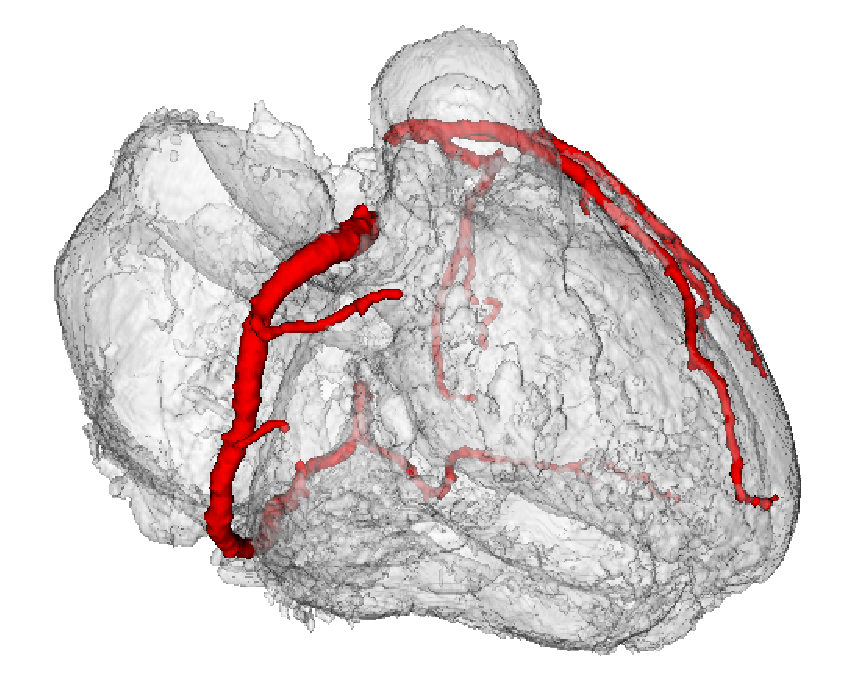
\includegraphics[height=1.5in]{../../Figures/gac/heart/heart_with_ca.eps}
% \caption[二值阈值后心脏区域前面观]{二值阈值后心脏区域前面观($\text{TH}_{\text{lower}} = 0$,$\text{TH}_{\text{upper}} = 200$)。注意其中的心包,以及大部分血管等都已被除去。}%
% \label{fig:heart_binary_threshold_experiments}
\end{figure}
\end{frame} 

\begin{frame}

\end{frame} 
 